\subsubsection{Barabel}
\begin{samepage}
    \begin{flushright}	
        \begin{tabular}{|l|r|}
            \textbf{Type}        & Reptile \\
            \textbf{Planète}     & Barab I \\
            \textbf{Langage}     & Barabel \\
            \textbf{Orientation} & Obscur \\
        \end{tabular}
    \end{flushright}

	\vspace{-5\baselineskip}
	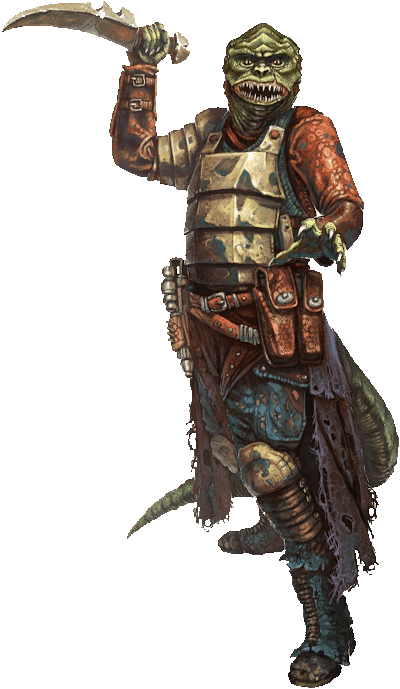
\includegraphics[width=5cm]{img/personnages/races/barabel.png}
\end{samepage}

Originaire de Barab I, les Barabels sont restés une race relativement primitive et isolée. Les Barabels vivent en clans dans un société principalement matriarcale. Ils sont fascinés par la guerre, la violence et les armes. Les Barabels ne sont pas profondément cruels, mais ils restent agressifs de nature. En raison des nombreux rituels précédent les négociations, la diplomatie avec les Barabels est un exercice compliqué.

Le Barabel adulte est un reptile bipède dont la taille dépasse toujours les deux mètres. Sa dentition est formée d’une multitude de dents en forme d’aiguilles qui peuvent atteindre jusqu’à cinq centimètres de long et ses mains sont équipées de griffes puissantes.

\begin{description}[align=left]
\item [Enfance difficile] 	% CAP +1 +1
		De par l’environnement hostile de leur planète natale, les Barabels possèdent une résistance accrue à la chaleur et aux radiations.\\
		\textit{+4 en Résistance à la chaleur}\\
		\textit{+4 en Résistance aux radiations}
\item [\OE{il} Ophidien] 	% CAP +1
		Les yeux ophidiens du Barabel lui permettent de capter la plupart des ondes lumineuses allant du jaune à l’infrarouge, mais il confond facilement les couleurs tirant dans les bleus et violets.\\
		\textit{Infravision}
\item [Arme naturelle]		% CAP +1
		Les mains des Barabels sont équipés de puissante griffes.\\
		\textit{For + d6 de dégâts}
\item [Balayage]			% CAP +2
		Les Barabels utilise leur appendice caudal d’instinct dans les combats.\\
		\textit{+ Atout Balayage}
\item [Primitif]			% CAP -3
		Les Barabels sont une race encore primitive.\\
		\textit{Int <= d6}
\item [Dur d’oreille]		% CAP -1
		Les Barabels en tant que reptilien ne possède pas d’oreille, ils entendent par vibrations.\\
		\textit{Dur d’oreille (Mineur)}
\end{description}
\newpage